\documentclass[12pt,letterpaper]{article}
\usepackage{graphicx,textcomp}
\usepackage{natbib}
\usepackage{setspace}
\usepackage{fullpage}
\usepackage{color}
\usepackage[reqno]{amsmath}
\usepackage{amsthm}
\usepackage{fancyvrb}
\usepackage{amssymb,enumerate}
\usepackage[all]{xy}
\usepackage{endnotes}
\usepackage{lscape}
\newtheorem{com}{Comment}
\usepackage{float}
\usepackage{hyperref}
\newtheorem{lem} {Lemma}
\newtheorem{prop}{Proposition}
\newtheorem{thm}{Theorem}
\newtheorem{defn}{Definition}
\newtheorem{cor}{Corollary}
\newtheorem{obs}{Observation}
\usepackage[compact]{titlesec}
\usepackage{dcolumn}
\usepackage{tikz}
\usetikzlibrary{arrows}
\usepackage{multirow}
\usepackage{xcolor}
\newcolumntype{.}{D{.}{.}{-1}}
\newcolumntype{d}[1]{D{.}{.}{#1}}
\definecolor{light-gray}{gray}{0.65}
\usepackage{url}
\usepackage{listings}
\usepackage{color}

\definecolor{codegreen}{rgb}{0,0.6,0}
\definecolor{codegray}{rgb}{0.5,0.5,0.5}
\definecolor{codepurple}{rgb}{0.58,0,0.82}
\definecolor{backcolour}{rgb}{0.95,0.95,0.92}

\lstdefinestyle{mystyle}{
	backgroundcolor=\color{backcolour},   
	commentstyle=\color{codegreen},
	keywordstyle=\color{magenta},
	numberstyle=\tiny\color{codegray},
	stringstyle=\color{codepurple},
	basicstyle=\footnotesize,
	breakatwhitespace=false,         
	breaklines=true,                 
	captionpos=b,                    
	keepspaces=true,                 
	numbers=left,                    
	numbersep=5pt,                  
	showspaces=false,                
	showstringspaces=false,
	showtabs=false,                  
	tabsize=2
}
\lstset{style=mystyle}
\newcommand{\Sref}[1]{Section~\ref{#1}}
\newtheorem{hyp}{Hypothesis}

\title{Problem Set 1}
\date{Due: January 29, 2020}
\author{QTM 200: Applied Regression Analysis}

\begin{document}
	\maketitle
	
	\section*{Instructions}
	\begin{itemize}
		\item Please show your work! You may lose points by simply writing in the answer. If the problem requires you to execute commands in \texttt{R}, please include the code you used to get your answers. Please also include the \texttt{.R} file that contains your code. If you are not sure if work needs to be shown for a particular problem, please ask.
		\item Your homework should be submitted electronically on the course GitHub page in \texttt{.pdf} form.
		\item This problem set is due at the beginning of class on Wednesday, January 22, 2020. No late assignments will be accepted.
		\item Total available points for this homework is 100.
	\end{itemize}
	
	\vspace{1cm}
	\section*{Question 1 (25 points)}
	
	A private school counselor was curious about the average of IQ of the students in her school and took a random sample of 25 students' IQ scores. The following is the data set:
	\vspace{.5cm}
	
	\lstinputlisting[language=R, firstline=40, lastline=40]{PS1.R}  
	\vspace{.5cm}
	
	\noindent Find a 90\% confidence interval for the student IQ in the school assuming the population of IQ from which our random sample has been selected is normally distributed. 
	
	\vspace{1cm}
	
	\lstinputlisting[language=R, firstline=43, lastline=50]{PS1_Answer.R}  
	
	\vspace{.5cm}
The confidence interval is (93.96, 102.92). Therefore, we're 90 percent confident that the true mean will fall within the interval of (93.96, 102.92).	
	\vspace{1cm}
		
	\section*{Question 2 (25 points)}
	A private school counselor was curious  whether  the average of IQ of the students in her school is higher than the average IQ score 100 among all the schools in the country. She took a random sample of 25 students' IQ scores. The following is the data set:
	\vspace{.5cm}
	\lstinputlisting[language=R, firstline=46, lastline=46]{PS1.R}  
	\vspace{.5cm}
	
	\noindent Conduct a test with 0.05 significance level assuming the population of IQ from which our random sample has been selected is normally distributed. 
	
	\vspace{1cm}
	
    \lstinputlisting[language=R, firstline=58, lastline=59]{PS1_Answer.R}
    \vspace{.5cm}
    
    I fail to reject the null hypothesis because p-value = 0.557, which is greater than 0.05.
    The average IQ of the school does not significantly differ from 100 on average.
    \vspace{1cm}
	
	
	\section*{Question 3 (50 points)}
	
	\noindent Researchers are curious about what affects the education expenditure on public education. The following is availabe variables in a data set about the education expenditure. \\
	\vspace{.5cm}
	
	
	\begin{tabular}{r|l}
		\texttt{State} &\emph{50 states in US} \\
		\texttt{Y} & \emph{per capita expenditure on public education}\\
		\texttt{X1} &\emph{per capita personal income} \\
		\texttt{X2} &  \emph{Number of residents per thousand under 18 years of age}\\
		\texttt{X3} &  \emph{Number of people per thousand residing in urban areas} \\
		\texttt{Region} &  \emph{1=Northeast, 2= North Central, 3= South, 4=West} \\
	\end{tabular}
	
	\vspace{.5cm}
	\noindent Explore the \texttt{expenditure} data set and import data into \texttt{R}.
	\vspace{.5cm}
	\lstinputlisting[language=R, firstline=54, lastline=54]{PS1.R}  
	\vspace{.5cm}
	\begin{itemize}
		
		\item
		Please plot the relationships among \emph{Y}, \emph{X1}, \emph{X2}, and \emph{X3}? What are the correlations among them (you just need to describe the graph and the relationships among them)?
		\vspace{.5cm}
		
		\lstinputlisting[language=R, firstline=71, lastline=73]{PS1_Answer.R}  
		\vspace{.5cm}
		\begin{figure}\centering
		\caption{Figure 1:Personal Income and Educational Expenditure}
		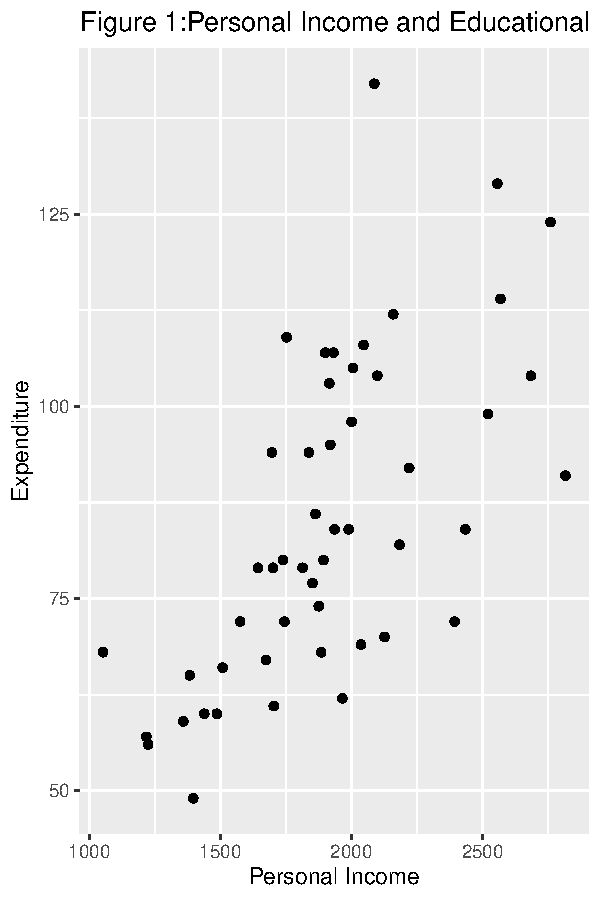
\includegraphics[width=0.85\textwidth]{Rplot1.pdf}
	    \end{figure}	
		The graph shows that as the per capita personal income increases, per capita expenditure on public education increases.
		\vspace{.5cm}
		
		\lstinputlisting[language=R, firstline=76, lastline=78]{PS1_Answer.R}  
		\vspace{.5cm}
		\begin{figure}\centering
			\caption{Figure 2:People under 18 and Educational Expenditure}
			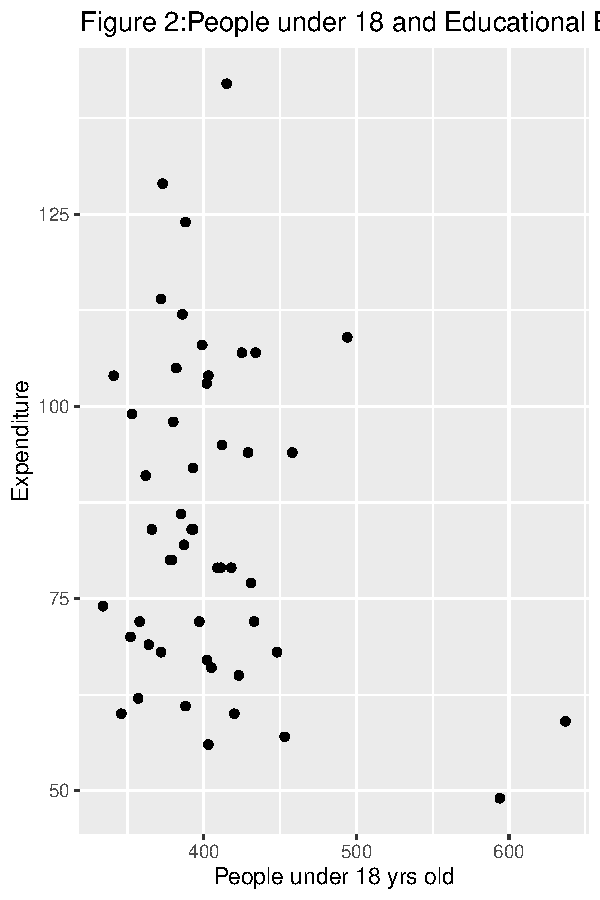
\includegraphics[width=0.85\textwidth]{Rplot2.pdf}
		\end{figure}
		The graph does not show a clear relationship between the number of residents under 18 years of age and the per capita expenditure on public education.
		\vspace{.5cm}
		
		\lstinputlisting[language=R, firstline=81, lastline=83]{PS1_Answer.R}  
		\vspace{.5cm}
	    \begin{figure}\centering
			\caption{Figure 3:People in urban area and Educational Expenditure}
			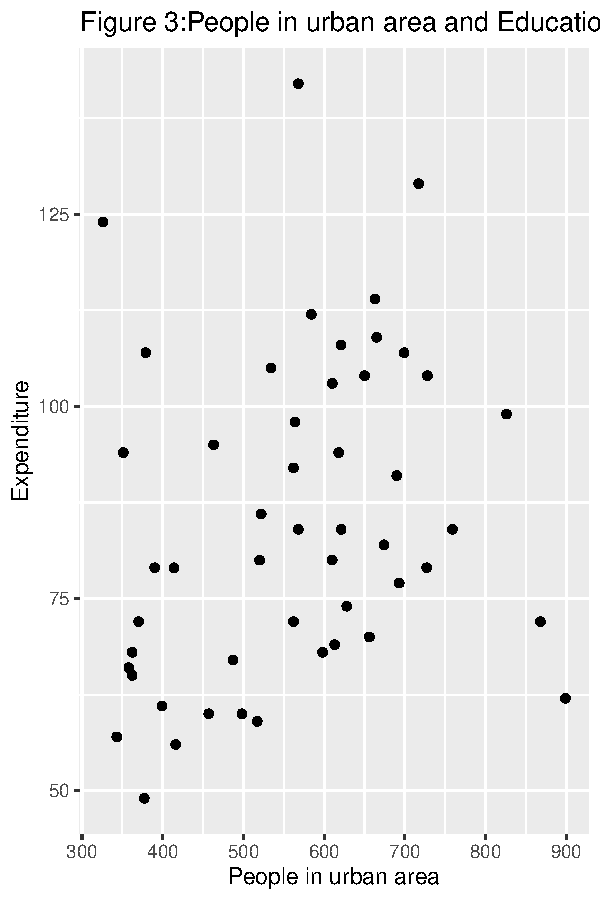
\includegraphics[width=0.85\textwidth]{Rplot3.pdf}
	     \end{figure}
		The graph shows that as the number of people residing in urban areas increases, per capita expenditure on public education increases.
		\vspace{.5cm}	
		
		\item
		Please plot the relationship between \emph{Y} and \emph{Region}? On average, which region has the highest per capita expenditure on public education?
		\vspace{.5cm}
			\lstinputlisting[language=R, firstline=87, lastline=87]{PS1_Answer.R}  
		\vspace{.5cm}
	    \begin{figure}\centering
		\caption{Figure 4:Region and Educational Expenditure}
		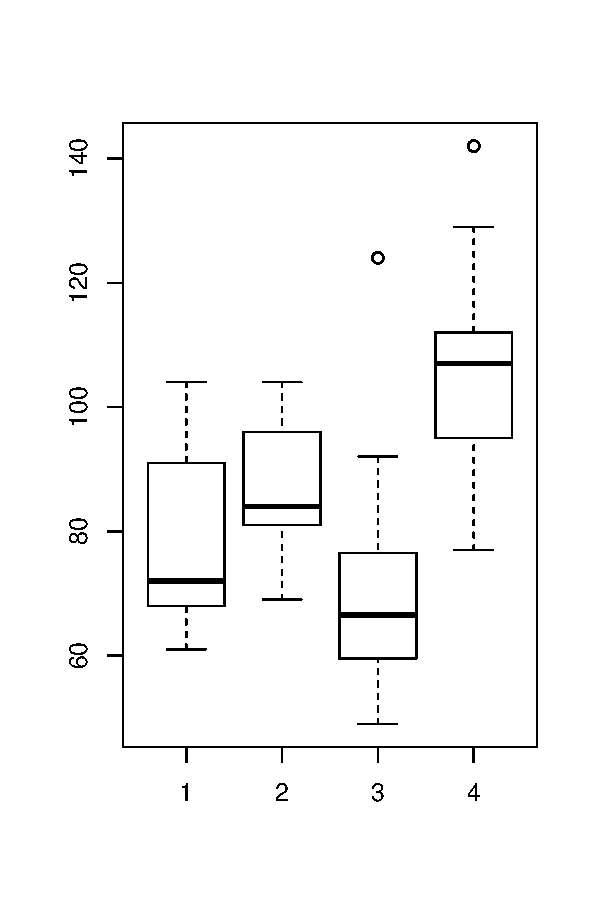
\includegraphics[width=0.85\textwidth]{Rplot4.pdf}
	 \end{figure}	
		The west has the highest per cpita expenditure on public education.
		
		\item
		Please plot the relationship between \emph{Y} and \emph{X1}? Describe this graph and the relationship. Reproduce the above graph including one more variable \emph{Region} and display different regions with different types of symbols and colors.
		\vspace{.5cm}
		\lstinputlisting[language=R, firstline=91, lastline=94]{PS1_Answer.R}  
		\vspace{.5cm}
	       \begin{figure}\centering
	       	\caption{Figure 5:Personal Income by Region and Educational Expenditure}
	       	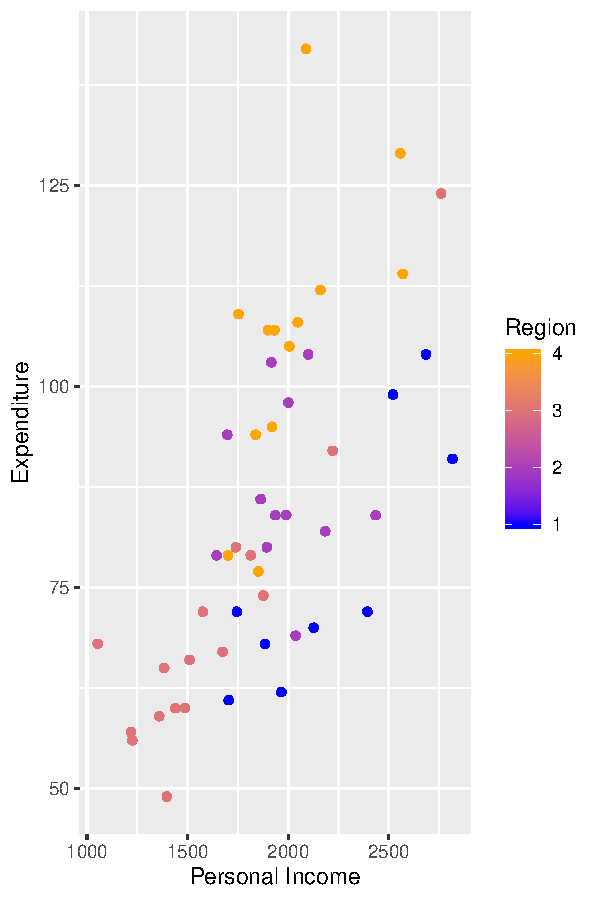
\includegraphics[width=0.95\textwidth]{Rplot5.pdf}
            \end{figure}	
		People with higher income in the Northeast and West are more likely to spend more on public education.
		Whilst people in the North Central and South do not spend more on public education if they earn higher income. 
		
	\end{itemize}
	
\end{document}
